\documentclass{beamer}
\usepackage{listings}
\usepackage{hyperref,animate}
\usepackage{tikz}
\usetikzlibrary{positioning,shadows,arrows,shapes,calc}
\def\labelenumi\theenumi
\usepackage{graphicx}
\usepackage{amsmath}
\mode<presentation>{\usetheme{Frankfurt}}
\AtBeginSection
{
  \begin{frame}<beamer>
    \frametitle{Outline}
    \tableofcontents[currentsection,currentsubsection]
  \end{frame}
}
\title{Partial and Total Derivatives}
\author{Mark Hasegawa-Johnson\\All content~\href{https://creativecommons.org/licenses/by-sa/4.0/}{CC-SA 4.0} unless otherwise specified.}
\date{ECE 417: Multimedia Signal Processing, Fall 2020}  
\titlegraphic{\includegraphics{../../../17fall/lectures/imark_1867_bold.png}}
\begin{document}

% Title
\begin{frame}
  \maketitle
\end{frame}

% Title
\begin{frame}
  \tableofcontents
\end{frame}

%%%%%%%%%%%%%%%%%%%%%%%%%%%%%%%%%%%%%%%%%%%%%%%%%%%%%%%%%
\section[FIR/IIR]{Linear Time Invariant Filtering: FIR \& IIR}
\setcounter{subsection}{1}

\begin{frame}
  \frametitle{Basics of DSP: Filtering}
  \[
  y[n] = \sum_{m=-\infty}^\infty h[m] x[n-m]
  \]
  \[
  Y(z)=H(z)X(z)
  \]
\end{frame}

\begin{frame}
  \frametitle{Finite Impulse Response (FIR)}
  \[
  y[n] = \sum_{m=0}^{N-1}h[m]x[n-m]
  \]
  The coefficients, $h[m]$, are chosen in order to optimally position
  the $N-1$ zeros of the transfer function, $r_k$, defined according to:
  \[
  H(z)=\sum_{m=0}^{N-1}h[m] z^{-m}=h[0]\prod_{k=1}^{N-1}\left(1-r_kz^{-1}\right)
  \]
\end{frame}

\begin{frame}
  \frametitle{Infinite Impulse Response (IIR)}
  \[
  y[n] = \sum_{m=0}^{N-1}b_mx[n-m] + \sum_{m=1}^{M-1}a_m y[n-m]
  \]
  The coefficients, $b_m$ and $a_m$, are chosen in order to optimally
  position the $N-1$ zeros and $M-1$ poles of the transfer function,
  $r_k$ and $p_k$, defined according to:
  \[
  H(z)=\frac{\sum_{m=0}^{N-1}b_m z^{-m}}{1-\sum_{m=1}^{M-1}a_m z^{-m}}
  =b_0\frac{\prod_{k=1}^{N-1}\left(1-r_kz^{-1}\right)}{\prod_{k=1}^{M-1}\left(1-p_kz^{-1}\right)}
  \]
  {\bf STABILITY:} If any of the poles are on or outside the unit
  circle ($|p_k|\ge 1$), then $y[n]\rightarrow\infty$, even with
  finite $x[n]$.
\end{frame}

%%%%%%%%%%%%%%%%%%%%%%%%%%%%%%%%%%%%%%%%%%%%%%%%%%%%%%%%%
\section[CNN/RNN]{Nonlinear Time Invariant Filtering: CNN \& RNN}
\setcounter{subsection}{1}

\begin{frame}
  \frametitle{Convolutional Neural Net = Nonlinear(FIR)}
  \centerline{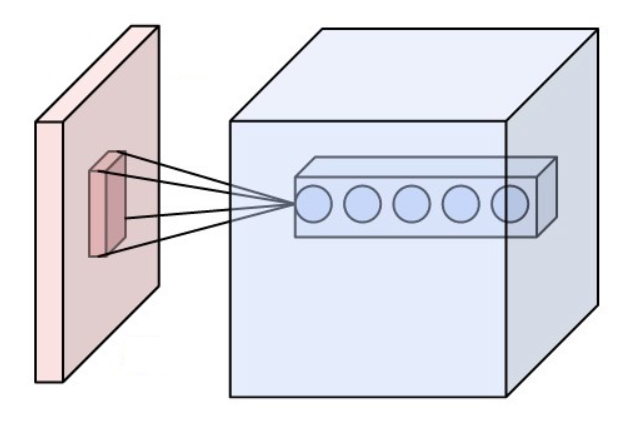
\includegraphics[height=1.5in]{exp/Conv_layer.png}}
  \begin{tiny}Image CC-SA-4.0  by Aphex34, \url{https://commons.wikimedia.org/wiki/File:Conv_layer.png}\end{tiny}
\end{frame}

\begin{frame}
  \frametitle{Convolutional Neural Net = Nonlinear(FIR)}
  \[
  \hat{y}[n] = g\left(\sum_{m=0}^{N-1}w[m]x[n-m]\right)
  \]
  The coefficients, $w[m]$, are chosen to minimize some kind of error.
  For example, suppose that the goal is to make $\hat{y}[n]$ resemble a
  target signal $y[n]$; then we might use 
  \[
  E = \frac{1}{2}\sum_{n=0}^N\left(\hat{y}[n]-y[n]\right)^2
  \]
  and choose
  \[
  w[n] \leftarrow w[n]-\eta\frac{dE}{dw[n]}
  \]
\end{frame}

\begin{frame}
  \frametitle{Recurrent Neural Net (RNN) = Nonlinear(IIR)}
  \centerline{\includegraphics[width=4.5in]{exp/800px-Recurrent_neural_network_unfold.svg.png}}
  \begin{tiny}Image CC-SA-4.0  by Ixnay, \url{https://commons.wikimedia.org/wiki/File:Recurrent_neural_network_unfold.svg}\end{tiny}
\end{frame}

\begin{frame}
  \frametitle{Recurrent Neural Net (RNN) = Nonlinear(IIR)}
  \[
  h[n] = g\left(x[n] + \sum_{m=1}^{M-1}w[m] h[n-m]\right)
  \]
  The coefficients, $w[m]$, are chosen to minimize the error.
  For example, suppose that the goal is to make $h[n]$ resemble a
  target signal $y[n]$; then we might use 
  \[
  E = \frac{1}{2}\sum_{n=0}^N\left(h[n]-y[n]\right)^2
  \]
  and choose
  \[
  w[m] \leftarrow w[m]-\eta\frac{dE}{dw[m]}
  \]
\end{frame}

%%%%%%%%%%%%%%%%%%%%%%%%%%%%%%%%%%%%%%%%%%%%%%%%%%%%%%%%%
\section[Partial Derivatives]{Partial and Total Derivatives}
\setcounter{subsection}{1}

\begin{frame}
  \frametitle{Partial Derivatives}

  In order to do back-propagation in recurrent neural networks, it
  will be important to distinguish between partial and total
  derivatives.  Unfortunately, these are not defined very clearly in
  introductory calculus classes.

  The standard definition of the partial derivative of $f(\vec{x})$
  w.r.t. $x_1$, where $\vec{x}=[x_1,\ldots,x_D]^T$, is
  \begin{displaymath}
    \frac{\partial f}{\partial x_1} = \lim_{\epsilon\rightarrow 0}\left(
    \frac{f(x_1+\epsilon,x_{2},\ldots)-f(x_1,x_{2},\ldots)}
         {\epsilon}\right)
  \end{displaymath}
\end{frame}
  
\begin{frame}
  \frametitle{Partial Derivatives}

  \begin{displaymath}
    \frac{\partial f}{\partial x_1} = \lim_{\epsilon\rightarrow 0}\left(
    \frac{f(x_1+\epsilon,x_{2},\ldots)-f(x_1,x_{2},\ldots)}
         {\epsilon}\right)
  \end{displaymath}

  In other words, $\frac{\partial f}{\partial x_k}$ is defined as the
  derivative of $f$ w.r.t. $x_k$ while holding all of the other $x_d$,
  for $1\le d\le D$, constant.
\end{frame}
\begin{frame}
  \frametitle{Total Derivatives}

  The partial derivative and total derivative differ if some of the
  {\bf other} elements of the vector $\vec{x}$ might depend on $x_k$.
  For example, suppose that each $x_j$ is a function of $x_i$ for $i\le j$:
  \begin{displaymath}
    x_j = g_j(x_1,\ldots,x_{j-1})
  \end{displaymath}
  Then the {\bf total} derivative allows each of the $x_j$, for $j>k$,
  to vary as $x_k$ varies:
  \begin{displaymath}
    \frac{d f}{d x_1} = \lim_{\epsilon\rightarrow 0}\left(
    \frac{f(x_1+\epsilon,x_{2}(x_1+\epsilon),\ldots)-
      f(x_1,x_{2}(x_1),\ldots)}{\epsilon}
    \right)
  \end{displaymath}
\end{frame}
  
\begin{frame}
  \frametitle{Partial and Total Derivatives}

  \begin{itemize}
  \item
    The {\bf partial derivative} of $f$ w.r.t. $x_k$ holds all of the
    other variables constant, while varying {\bf only} $x_k$.  The
    other variables are held constant {\bf ignoring any dependency
      they otherwise would have on} $x_k$:
    \begin{displaymath}
    \frac{\partial f}{\partial x_1} = \lim_{\epsilon\rightarrow 0}\left(
    \frac{f(x_1+\epsilon,x_{2}(x_1),\ldots)-
      f(x_1,x_{2}(x_1),\ldots)}{\epsilon}
    \right)
    \end{displaymath}
  \item
    The {\bf total derivative} takes into account the effect that
    varying $x_k$ might have on all the other variables:
    \begin{displaymath}
    \frac{d f}{d x_1} = \lim_{\epsilon\rightarrow 0}\left(
    \frac{f(x_1+\epsilon,x_{2}(x_1+\epsilon),\ldots)-
      f(x_1,x_{2}(x_1),\ldots)}{\epsilon}
    \right)
    \end{displaymath}
  \end{itemize}
\end{frame}

\begin{frame}
  \frametitle{Partial and Total Derivatives}

  \begin{itemize}
    \item So far, we've pretended that, when we say ``holding all
      other variables constant,'' we know what that means.
    \item In a neural network, there are lots of implicit variables,
      that you can calculate if you want to.
    \item When you say ``holding all other variables constant,'' it is
      necessary to specify exactly which other variables you mean.
  \end{itemize}
\end{frame}

%%%%%%%%%%%%%%%%%%%%%%%%%%%%%%%%%%%%%%%%%%%%%%%%%%%%%%%%%
\section[Back-Prop]{Back-Propagation Review}
\setcounter{subsection}{1}

\begin{frame}
  \frametitle{Review: Excitation and Activation}
  \begin{itemize}
    \item The {\bf\em activation} of a hidden node is the output of
      the nonlinearity (for this reason, the nonlinearity is sometimes
      called the {\bf activation function}).  For example, in a
      fully-connected network with outputs $\hat{y}_l$, weights $\vec{w}$,
      bias $b$, nonlinearity $g()$, and hidden node activations
      $\vec{h}$, the activation of the $l^{\textrm{th}}$ output node
      is
      \[
      \hat{y}_l = g\left(b_{l}+\sum_{k=1}^p w_{lk} h_k\right)
      \]
    \item The {\bf\em excitation} of a hidden node is the input of the
      nonlinearity.  For example, the excitation of the node above is
      \[
      \xi_l=b_{l}+\sum_{k=1}^p w_{lk} h_k
      \]
  \end{itemize}
\end{frame}

\begin{frame}
  \frametitle{Backprop = Derivative w.r.t. Excitation}
  \begin{itemize}
    \item The {\bf\em excitation} of a hidden node is the input of the
      nonlinearity.  For example, the excitation of the node above is
      \[
      \xi_l = b_{l}+\sum_{k=1}^p w_{lk} h_k
      \]
    \item The gradient of the error w.r.t. the weight is
      \[
      \frac{d{\mathcal L}}{d w_{lk}} = \epsilon_lh_k
      \]
      where $\epsilon_l$ is the derivative of the error w.r.t. the
      $l^{\textrm{th}}$ {\bf\em excitation}:
      \[
      \epsilon_l = \frac{d{\mathcal L}}{de_l}
      \]
  \end{itemize}
\end{frame}

\begin{frame}
  \frametitle{Backprop for Fully-Connected Network}

  Suppose we have a fully-connected network, with inputs $\vec{x}$,
  weight matrices $W^{(1)}$ and $W^{(2)}$, nonlinearities $g()$ and
  $h()$, and output $\hat{y}$:
  \begin{align*}
    \xi_k^{(1)} = b_{k}^{(1)}+\sum_j w_{kj}^{(1)} x_j,&~~~~
    h_k = g\left(\xi_k^{(1)}\right)\\
    \xi_l^{(2)} = b_{l}^{(2)}+\sum_k w_{lk}^{(2)} h_k,&~~~~
    \hat{y}_l = h\left(\xi_l^{(2)}\right)
  \end{align*}
  Then the back-prop gradients are the derivatives of ${\mathcal L}$ with respect
  to the {\bf\em excitations} at each node:
  \begin{align*}
    \frac{d{\mathcal L}}{dw_{lk}^{(2)}} =\epsilon_lh_k,&~~~~\epsilon_l=\frac{d{\mathcal L}}{d\xi_l^{(2)}}\\
      \frac{d{\mathcal L}}{dw_{kj}^{(1)}}=\delta_kx_j,&~~~~\delta_k=\frac{d{\mathcal L}}{d\xi_k^{(1)}}
  \end{align*}
\end{frame}

\begin{frame}
  \frametitle{Back-Prop Example}

  Suppose we have the following network:
  \begin{align*}
    h &= \cos(x)\\
    \hat{y} &= \sqrt{1+h^2}
  \end{align*}
  Suppose we need $\frac{d\hat{y}}{dx}$.  We find it as
  \begin{align*}
    \frac{d\hat{y}}{dx} &= \frac{d\hat{y}}{dh}\frac{\partial h}{\partial x}
    = \left(\frac{h}{\sqrt{1+h^2}}\right)\left(-\sin(x)\right)
  \end{align*}    
\end{frame}

\begin{frame}
  \frametitle{Back-Prop Example}

  Suppose we have the following network:
  \begin{align*}
    h_0 &= \cos(x)\\
    h_1 &= \frac{1}{\sqrt{2}}\left(h_0^3+\sin(x)\right)\\
    \hat{y} &= \sqrt{h_0^2+h_1^2}
  \end{align*}
  What  is $\frac{d\hat{y}}{dx}$?  How can we compute that?
\end{frame}

\begin{frame}
  \frametitle{Flow Graphs}

  \centerline{
    \tikzstyle{pre}=[<-,shorten <=1pt,>=stealth',semithick,draw=blue]
    \begin{tikzpicture}[hoop/.style={circle,thick,draw=blue,text=black,
          fill=orange!35!white,text centered,text width=0.25cm}]
      \node[hoop] (x) at (0,0) {$x$};
      \node[hoop] (h0) at (-2,1) {$h_0$} edge[pre] (x);
      \node[hoop] (h1) at (2,2) {$h_1$} edge[pre] (x) edge[pre](h0);
      \draw[dashed] (-2.5,0.5) -- (2.5,0.5);
      \node[hoop] (yhat) at (0,3) {$\hat{y}$} edge[pre](h0) edge[pre](h1);
  \end{tikzpicture}}

  We often show the flow graph for the chain rule using bubbles and
  arrows, as shown above.  You can imagine the chain rule as taking a
  summation along any cut through the flow graph---for example, the
  dashed line shown above.  You take the total derivative from
  $\hat{y}$ to the cut, and then the partial derivative from there
  back to $x$.
  \begin{displaymath}
    \frac{d\hat{y}}{dx} = \sum_{i=0}^{N-1}\frac{d\hat{y}}{dh_i}\frac{\partial h_i}{\partial x}
  \end{displaymath}
\end{frame}


\begin{frame}
  \frametitle{Flow Graphs}

  \centerline{
    \tikzstyle{pre}=[<-,shorten <=1pt,>=stealth',semithick,draw=blue]
    \begin{tikzpicture}[hoop/.style={circle,thick,draw=blue,text=black,
          fill=orange!35!white,text centered,text width=0.25cm}]
      \node[hoop] (x) at (0,0) {$x$};
      \node[hoop] (h0) at (-2,1) {$h_0$} edge[pre] (x);
      \node[hoop] (h1) at (2,2) {$h_1$} edge[pre] (x) edge[pre](h0);
      \draw[dashed] (-2.5,0.5) -- (2.5,0.5);
      \node[hoop] (yhat) at (0,3) {$\hat{y}$} edge[pre](h0) edge[pre](h1);
  \end{tikzpicture}}
  \begin{displaymath}
    \frac{d\hat{y}}{dx} = \sum_{i=0}^{N-1}\frac{d\hat{y}}{dh_i}\frac{\partial h_i}{\partial x}
  \end{displaymath}
  For each $h_i$, we find the {\bf total derivative} of $\hat{y}$
  w.r.t. $h_i$, multiplied by the {\bf partial derivative} of $h_i$ w.r.t. $x$.
\end{frame}

\begin{frame}
  \frametitle{Back-Prop Example}

  First, we find $\frac{d\hat{y}}{dh_1}$:
  \begin{align*}
    \hat{y} &= \sqrt{h_0^2+h_1^2}
  \end{align*}
  \begin{align*}
    \frac{d\hat{y}}{dh_1} &= \frac{h_1}{\sqrt{h_0^2+h_1^2}}
  \end{align*}
\end{frame}

\begin{frame}
  \frametitle{Back-Prop Example}

  \centerline{
    \tikzstyle{pre}=[<-,shorten <=1pt,>=stealth',semithick,draw=blue]
    \begin{tikzpicture}[hoop/.style={circle,thick,draw=blue,text=black,
          fill=orange!35!white,text centered,text width=0.25cm}]
      \node[hoop] (x) at (0,0) {$x$};
      \node[hoop] (h0) at (-2,1) {$h_0$} edge[pre] (x);
      \node[hoop] (h1) at (2,2) {$h_1$} edge[pre] (x) edge[pre](h0);
      \draw[dashed] (-2.5,1.5) -- (1.5,1.5);
      \node[hoop] (yhat) at (0,3) {$\hat{y}$} edge[pre](h0) edge[pre](h1);
  \end{tikzpicture}}
  Second, back-prop to find $\frac{d\hat{y}}{dh_0}$:
  \begin{align*}
    \frac{d\hat{y}}{dh_0} &=\frac{\partial\hat{y}}{\partial h_0}
    + \frac{d\hat{y}}{d h_1}\frac{\partial h_1}{\partial h_0}
    = \frac{1}{\sqrt{h_0^2+h_1^2}}\left(h_0+\left(\frac{3}{\sqrt{2}}\right)h_0^2h_1\right)
  \end{align*}
\end{frame}

\begin{frame}
  \frametitle{Back-Prop Example}

  \centerline{
    \tikzstyle{pre}=[<-,shorten <=1pt,>=stealth',semithick,draw=blue]
    \begin{tikzpicture}[hoop/.style={circle,thick,draw=blue,text=black,
          fill=orange!35!white,text centered,text width=0.25cm}]
      \node[hoop] (x) at (0,0) {$x$};
      \node[hoop] (h0) at (-2,1) {$h_0$} edge[pre] (x);
      \node[hoop] (h1) at (2,2) {$h_1$} edge[pre] (x) edge[pre](h0);
      \draw[dashed] (-2.5,0.5) -- (2.5,0.5);
      \node[hoop] (yhat) at (0,3) {$\hat{y}$} edge[pre](h0) edge[pre](h1);
  \end{tikzpicture}}
  Third, back-prop to find $\frac{d\hat{y}}{dx}$:
  \begin{align*}
    \frac{d\hat{y}}{dx} &=\frac{d\hat{y}}{dh_1}\frac{\partial h_1}{\partial x}
    + \frac{d\hat{y}}{d h_0}\frac{\partial h_0}{\partial x}\\
    &= \left(\frac{h_1}{\sqrt{h_0^2+h_1^2}}\right)\cos(x)
    - \left(\frac{\left(h_0+\left(\frac{3}{\sqrt{2}}\right)h_0^2h_1\right)}{\sqrt{h_0^2+h_1^2}}\right)
    \sin(x)
  \end{align*}
\end{frame}


\begin{frame}
  \frametitle{Back-Prop and Partial Derivativees}
  Suppose we have a neural net, defined by
  \begin{align*}
    \xi_k^{(l+1)} &= \sum_{j}w_{k,j}^{(l+1)}\sigma\left(\xi_j^{(l)}\right)
  \end{align*}
  then, if we define
  \[
  \delta_j^{(l)} = \frac{\partial{\mathcal L}}{\partial\xi_j^{(l)}}
  \]
  we can compute it as
  \[
  \delta_j^{(l)} = \sum_k\delta_k^{(l+1)}\left(\frac{\partial\xi_k^{(l+1)}}{\partial\xi_j^{(l)}}\right)
  \]
  Here, the partial-derivative sign $\partial$ means that we hold
  constant all other $\xi$ variables {\bf at the same layer}.  We're
  obviously not holding constant all excitations at the {\bf next}
  layer, because those are the things over which we compute the back-prop.
\end{frame}

%%%%%%%%%%%%%%%%%%%%%%%%%%%%%%%%%%%%%%%%%%%%%%%%%%%%%%%%%%%%%%%%%%%%%%%%%%%%%%%%%
\section{Conclusion}
\setcounter{subsection}{1}

\begin{frame}
  \frametitle{Conclusions}
  \begin{itemize}
  \item Back-Prop, in general, is just the chain rule of calculus:
    \begin{displaymath}
      \frac{d{\mathcal L}}{dw} = \sum_{i=0}^{N-1}\frac{d{\mathcal L}}{dh_i}\frac{\partial h_i}{\partial w}
    \end{displaymath}
  \item Convolutional Neural Networks are the nonlinear version of an FIR filter.
    Coefficients are shared across time steps.
  \item Recurrent Neural Networks are the nonlinear version of an IIR filter.  
    Coefficients are shared across time steps.
    Error is back-propagated from every output time step to every input time step.
  \end{itemize}
\end{frame}

%%%%%%%%%%%%%%%%%%%%%%%%%%%%%%%%%%%%%%%%%%%%%%%%%%%%%%%%%%%%%%%%%%%%%%%%%%%%%%%%%
\section[Example]{Written Example}
\setcounter{subsection}{1}

\begin{frame}
  \frametitle{Written Example}
  Consider a set of variables $(u,v,w,x,y,z)$ with the following relationships:
  \begin{align*}
    u &= \epsilon_u\\
    v &= 0.1 u+\epsilon_v\\
    w &= 0.1 v + 0.1 u + \epsilon_w\\
    x &= 0.1 w + 0.1 v + 0.1 u +\epsilon_x\\
    y &= 0.1 x + 0.1 w + 0.1 v+ 0.1 u+\epsilon_y\\
    z &= 0.1 y+ 0.1 x + 0.1 w + 0.1 v+ 0.1 u+\epsilon_z
  \end{align*}
  \begin{enumerate}
  \item Draw a flow-graph.
  \item Calculate the gradient of $z$ w.r.t. the vector $\vec\phi=[u,v]^T$.
  \end{enumerate}
\end{frame}
  

\end{document}

